\documentclass{beamer}

\usepackage[utf8]{inputenc}
\usepackage[T1]{fontenc}
\usepackage[english, italian]{babel}
\usepackage{tikz}

\setcounter{tocdepth}{1}

\definecolor{azzurro}{HTML}{E6E6FF}

\usetheme[compress]{Berlin}
\beamertemplatenavigationsymbolsempty

\title{Piattaforma di video streaming per assistenza da remoto su dispositivi wearable}
\author{Simone Barco}
\institute[Università degli Studi di Padova]
{
	Dipartimento di Matematica "Tullio Levi-Civita"\\
	Corso di Laurea in Informatica
}
\date{Padova, 27 febbraio 2018}


\begin{document}
	\begin{frame}[noframenumbering, plain]
		\titlepage
	\end{frame}

	\begin{frame}[noframenumbering]{Indice dei contenuti}
		\tableofcontents
	\end{frame}

	\addtobeamertemplate{navigation symbols}{}{%
		\usebeamerfont{footline}%
		\usebeamercolor[fg]{footline}%
		\hspace{1em}%
		\insertframenumber/\inserttotalframenumber
	}

	\section{Analisi del contesto aziendale}
	\subsection{}
		\begin{frame}{L'azienda ospitante}
			\begin{figure}[H]
				\centering
				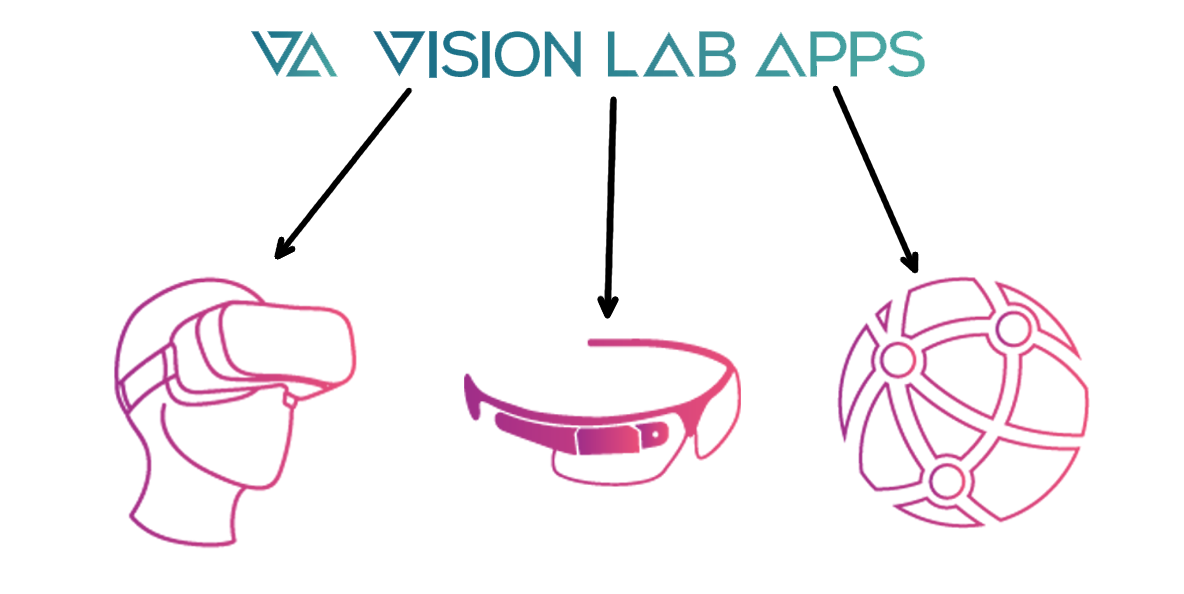
\includegraphics[width=1.0\textwidth]{capitolo_1/immagini/VLA.png}
			\end{figure}
		\end{frame}
	\subsection{}
		\begin{frame}{Progetti}
			\begin{itemize}
				\item \emph{VisioHealthCare}
				\begin{figure}[H]
					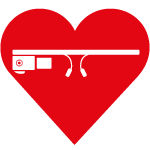
\includegraphics[width=0.2\textwidth]{capitolo_1/immagini/vhc.png}
				\end{figure}
				\item \emph{NapkinForever - Pininfarina Segno}
				\begin{figure}
					
\includegraphics[width=0.6\textwidth]{capitolo_1/immagini/forever.png}
				\end{figure}
			\end{itemize}
		\end{frame}

	\section{Presentazione dello stage}
	\subsection{}
		\begin{frame}{ERA - Enterprise Remote Assistance}
			\begin{minipage}{\textwidth}
				\begin{minipage}{0.60\textwidth}
					\begin{itemize}
						\item Ricevere istruzioni sulle attività da svolgere
						\item Eseguire passaggi e procedimenti operativi
						\item Condividere informazioni
						\item Offrire supporto in tempo reale
					\end{itemize}
				\end{minipage}
				\begin{minipage}{0.30\textwidth}
					\begin{figure}
						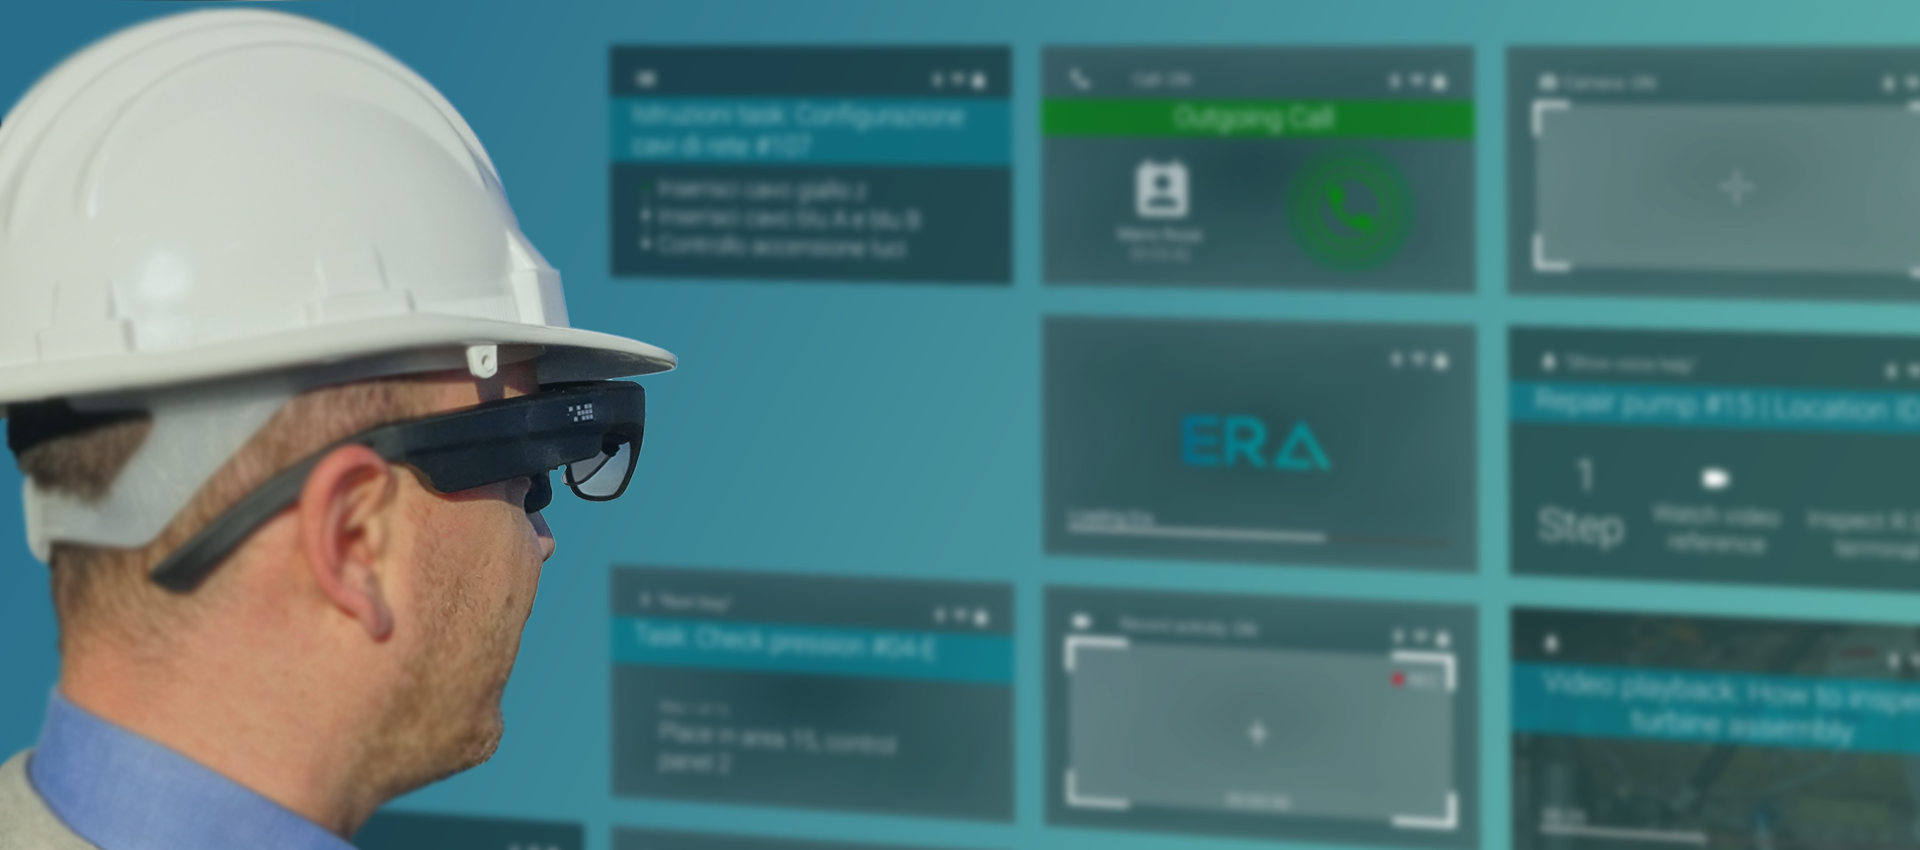
\includegraphics[width=1.5\textwidth]{capitolo_2/immagini/era.png}
					\end{figure}
				\end{minipage}
			\end{minipage}
		\end{frame}
	\subsection{}
		\begin{frame}{Tecnologie}
			\begin{center}
				\begin{minipage}{\textwidth}
					\begin{minipage}{0.29\textwidth}
						
\includegraphics[width=0.5\textwidth]{capitolo_2/immagini/java.png}
					\end{minipage}
					\begin{minipage}{0.60\textwidth}
						\begin{block}{\emph{Server Java}}
							\begin{itemize}
								\item Creazione e gestione canale di comunicazione
								\item Gestione utenti
								\item Sistema di autenticazione
							\end{itemize}
						\end{block}
					\end{minipage}
				\end{minipage}
				\vspace{2mm}
				\begin{minipage}{\textwidth}
					\begin{minipage}{0.60\textwidth}
						\begin{block}{\emph{Applicazione Android}}
							\begin{itemize}
								\item Prototipo lato \emph{client}
								\item Chat
								\item \emph{Streaming} audio-video
							\end{itemize}
						\end{block}
					\end{minipage}
					\begin{minipage}{0.29\textwidth}
							\begin{flushright}
								
\includegraphics[width=0.9\textwidth]{capitolo_2/immagini/android.png}
							\end{flushright}
					\end{minipage}
				\end{minipage}
			\end{center}
		\end{frame}

	\section{Svolgimento dello stage}
	\subsection{}
		\begin{frame}{Metodologia di lavoro}
			\begin{figure}
				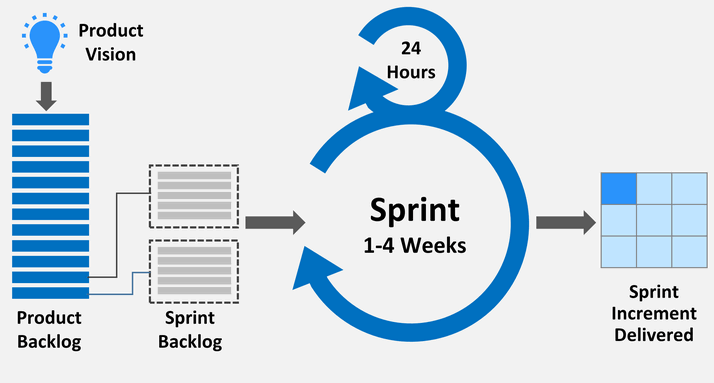
\includegraphics[width=0.99\textwidth]{capitolo_3/immagini/scrum.png}
			\end{figure}
		\end{frame}
	\subsection{}
		\begin{frame}{Analisi dei requisiti}
			\emph{Obbligatori}
				\begin{itemize}
							\item Creazione e gestione canale
							\item Implementazione utenti
							\item Sistema di permessi
				\end{itemize}
			\emph{Opzionali}
				\begin{itemize}
						\item Integrazione interfaccia grafica
						\item Unione con applicazione Android
				\end{itemize}
			\end{frame}
	\subsection{Sviluppo Server Java}
	\begin{frame}{Eclipse Vert.x}
		\begin{minipage}{0.5\textwidth}
			\emph{Vantaggi}
						\begin{itemize}
							\item alta scalabilità
							\item poliglotta
							\item documentazione
						\end{itemize}
			\emph{Costrutti fondamentali}
				\begin{itemize}
					\item Event Loop
					\item Event Bus
					\item Verticle
				\end{itemize}
			\end{minipage}
			\begin{minipage}{0.3\textwidth}
					\begin{figure}
						
\includegraphics[width=1.2\textwidth]{capitolo_3/immagini/Vertx.png}
					\end{figure}
				\end{minipage}
			\end{frame}
	\subsection{Sviluppo Server Java}
		\begin{frame}{Progettazione}
			\begin{minipage}{0.6\textwidth}
				\emph{Canale di comunicazione}
					\begin{itemize}
						\item Creazione ed eliminazione
						\item Invio e ricezione di \emph{messaggi}
						\item Aggiunta e rimozione \emph{utenti}
					\end{itemize}
			\end{minipage}
			\begin{minipage}{0.3\textwidth}
				\begin{figure}
					
\includegraphics[width=0.7\textwidth]{capitolo_3/immagini/comunicazione.png}
				\end{figure}
			\end{minipage}
			\begin{minipage}{0.6\textwidth}
				\emph{Utenti}
					\begin{itemize}
						\item Amministratore
						\item Utente Base
					\end{itemize}
			\end{minipage}
			\begin{minipage}{0.3\textwidth}
				\begin{figure}
					
\includegraphics[width=0.7\textwidth]{capitolo_3/immagini/utenti.jpg}
				\end{figure}
			\end{minipage}
			\begin{minipage}{0.6\textwidth}
				\emph{Sistema di autorizzazione}
				\begin{itemize}
					\item Lato Utente (richiesta)
					\item Lato Amministratore (autorizzazione/rimozione)
				\end{itemize}
			\end{minipage}
			\begin{minipage}{0.3\textwidth}
				\begin{figure}
					
\includegraphics[width=0.7\textwidth]{capitolo_3/immagini/autorize.jpg}
				\end{figure}
			\end{minipage}
		\end{frame}
	\subsection{Sviluppo Server Java}
		\begin{frame}{Implementazione}
			\begin{minipage}{0.4\textwidth}
				\emph{Canale di comunicazione}
					\begin{itemize}
						\item Messaggi $\rightarrow$ JSON
						\item EventBus $\rightarrow$ Vert.x
					\end{itemize}
			\end{minipage}
			\begin{minipage}{0.4\textwidth}
				\begin{figure}
					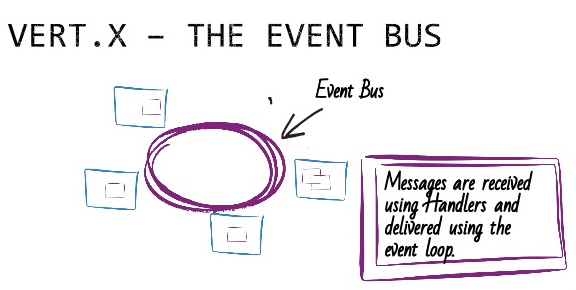
\includegraphics[width=1.6\textwidth]{capitolo_3/immagini/eventbus.jpg}
				\end{figure}
			\end{minipage}
			\begin{minipage}{0.3\textwidth}
				\emph{Utenti}
					\begin{itemize}
						\item User (interfaccia)
						\item UserBase
						\item Admin
					\end{itemize}
			\end{minipage}
			\begin{minipage}{0.5\textwidth}
				\emph{Sistema di autorizzazione}
				\begin{itemize}
					\item Utente $\rightarrow$ request()
					\item Amministratore $\rightarrow$ authorize(UserBase[])
				\end{itemize}
			\end{minipage}
		\end{frame}
	\subsection{}
		\begin{frame}{Interfaccia grafica}
			\begin{minipage}{0.4\textwidth}
				\begin{block}{Moduli utilizzati}
					\begin{itemize}
						\item Vert.x HTTPServer
						\item Vert.x WebSocket
					\end{itemize}
				\end{block}
			\end{minipage}
			\begin{minipage}{0.5\textwidth}
				\begin{figure}
					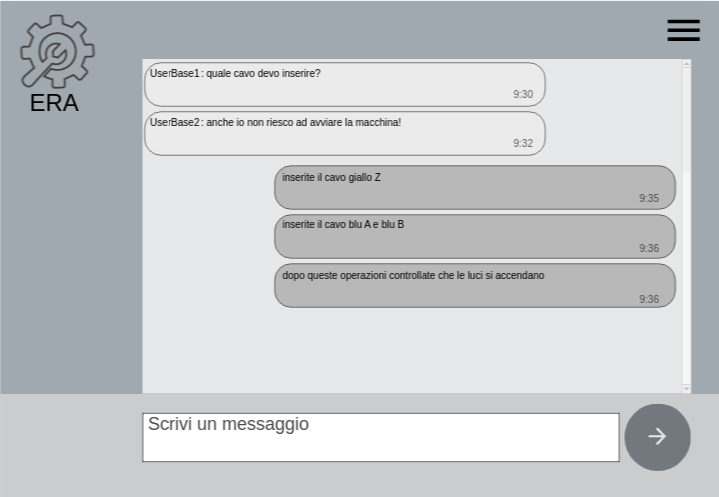
\includegraphics[width=1.2\textwidth]{capitolo_3/immagini/chat.png}
				\end{figure}
			\end{minipage}
			\begin{minipage}{0.3\textwidth}
				\begin{figure}
					
\includegraphics[width=0.5\textwidth]{capitolo_3/immagini/js.png}
				\end{figure}
			\end{minipage}
			\begin{minipage}{0.4\textwidth}
				\begin{block}{Funzioni}
					\begin{itemize}
						\item invio e ricezione
						\item autorizzazione
					\end{itemize}
				\end{block}
			\end{minipage}
		\end{frame}

	\section{Resoconto retrospettivo}
	\subsection{}
		\begin{frame}{Principali problemi}
			\begin{minipage}{0.6\textwidth}
				\begin{block}{Ecplise Vert.x}
					\begin{itemize}
						\item molti moduli
						\item \emph{community} limitata
					\end{itemize}
				\end{block}
			\end{minipage}
			\begin{minipage}{0.3\textwidth}
				\begin{figure}
					
\includegraphics[width=0.5\textwidth]{capitolo_4/immagini/problema.jpg}
				\end{figure}
			\end{minipage}
			\begin{minipage}{0.3\textwidth}
				\begin{figure}
					
\includegraphics[width=0.5\textwidth]{capitolo_4/immagini/problema2.png}
				\end{figure}
			\end{minipage}
			\begin{minipage}{0.6\textwidth}
				\begin{block}{Metodo di lavoro}
					\begin{itemize}
						\item difficoltà iniziale con \emph{Scrum}
					\end{itemize}
				\end{block}
			\end{minipage}
		\end{frame}
	\subsection{}
		\begin{frame}{Riassunto finale}
			\begin{minipage}{0.6\textwidth}
				\emph{Obiettivi raggiunti}
				\begin{itemize}
					\item Requisiti obbligatori: 3/3
					\item Requisiti opzioniali: 1/2
					\item Verifica: test soddisfacenti
					\item Validazione interna
				\end{itemize}
			\end{minipage}
			\begin{minipage}{0.3\textwidth}
				\begin{figure}
					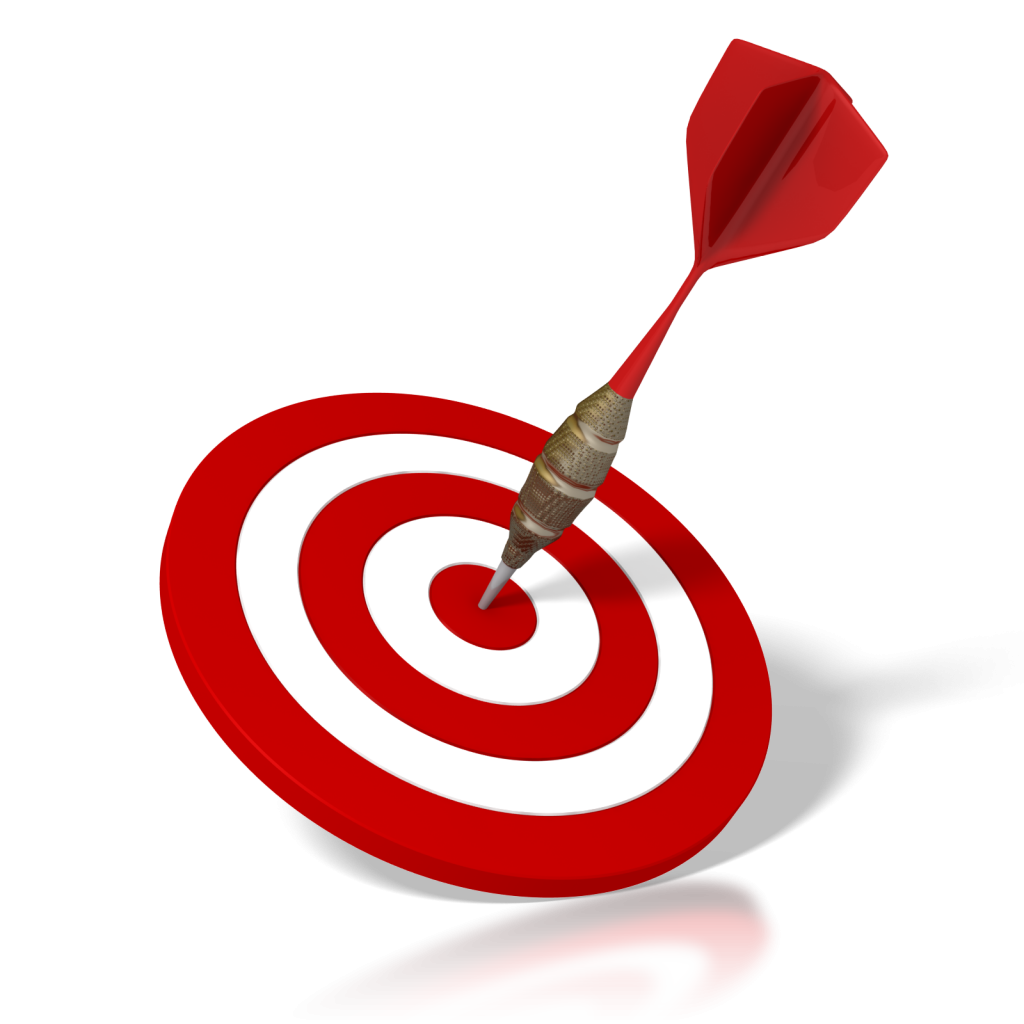
\includegraphics[width=0.9\textwidth]{capitolo_4/immagini/obiettivo.png}
				\end{figure}
			\end{minipage}
			\begin{minipage}{0.3\textwidth}
				\begin{figure}
					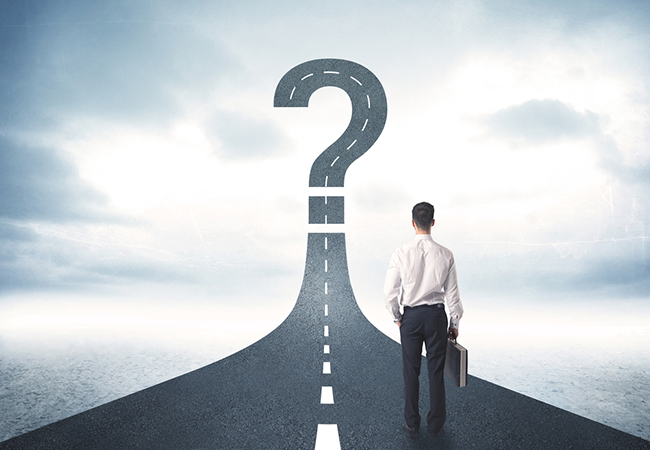
\includegraphics[width=1.0\textwidth]{capitolo_4/immagini/futuro}
				\end{figure}
			\end{minipage}
			\begin{minipage}{0.6\textwidth}
				\emph{Sviluppi futuri}
				\begin{itemize}
					\item Integrazione applicazione Android
					\item Tracking oggetti
				\end{itemize}
			\end{minipage}
		\end{frame}

\end{document}
